\chapter{Założenia projektowe}
\label{ch:zalozenia_projektowe}

W~przypadku projektowania programu komputerowego, istotne są założenia dla części technicznej oraz funkcjonalnej.
Założenia techniczne określają, jakie technologie i~narzędzia zostaną wykorzystane do stworzenia aplikacji,
jak~również zastosowane wzorce projektowe oraz architekturę.
Założenia funkcjonalne natomiast mają na celu zdefiniowanie, jakie funkcje i~mechanizmy powinny zostać zaimplementowane
oraz przede wszystkim, jak~te~funkcje pomogą spełnić cel aplikacji.

\section{Założenia funkcjonalne}
\label{sec:zalozenia_funkcjonalne}

Najistotniejsze podczas projektowania programu są założenia funkcjonalne,
które tak naprawdę definiują późniejsze założenia techniczne oraz samo działanie aplikacji.
Założenia te definiują obszary takie jak~interfejs użytkownika, mechanizmy oraz wprowadzanie danych wejściowych.\\
\indent Głównym celem aplikacji jest umożliwienie użytkownikowi projektowanie prostych schematów układów scalonych.
Wymaga to zaimplementowania edytora graficznego będącego w~stanie przedstawić przystępnie topografię układu scalonego.
Najbardziej intuicyjne jest wykorzystanie podejścia opierającego się na rysowaniu komórek,
które składałyby się w~elementy tworzące schemat, podobnie jak~to ma miejsce w~programach Magic VLSI czy Microwind.
Aby wprowadzić podstawowe założenia projektowania układu scalonego, oparto je o technologie Amis C5,
opracowane przez firmę Mosis.
Technologia ta definiuje rzeczywiste wymiary każdej kwadratowej komórki poprzez parametr $\lambda$
zawarty w~regułach projektowania.
Sam wybór jakiejkolwiek technologii projektowania podyktowany
jest próbą nauczenia skalowania wymiarów komórek względem wymiarów rzeczywistych.
Jedne z~takich reguł projektowania to \textit{SCMOS\_SUBM} o $\lambda=0,3~\um$~\cite{amis_c5, amis_params}.
Definiują one również dostępne materiały, z~których może się składać układ, parametry elementów oraz ograniczenia.
Podstawowe materiały przedstawiono w~tab.~\ref{tab:amis_materials}.
Wybór tych materiałów powinien odbywać się poprzez paletę warstw,
dzięki czemu użytkownik może w~sposób prosty wybrać odpowiedni z~nich,
jednocześnie mając przegląd wszystkich dostępnych warstw. 
%Zasady projektowania wskazują także najmniejsze dopuszczalne tranzystory: 3,0\um \times 0,6\um (W/L)~\cite{amis_params}.,
%czyli po podzieleniu przez $\lambda$ otrzymujemy 10 \times 2.

\newpage
\begin{table}[h]
    \centering
    \caption[Dostępne materiały w~technologii Amis C5.]
    {Dostępne podstawowe materiały w~technologii Amis C5, źródło:~\cite{amis_params}.}
    \label{tab:amis_materials}
    \begin{tabular}{|l|l|}
        \hline
        Nazwa materiału & Opis \\
        \hline
        \hline
        \texttt{substrate} & podłoże \\
        \hline
        \texttt{N+active} & inaczej \texttt{ndiffusion}, krzem typu n\\
        \hline
        \texttt{P+active} & inaczej \texttt{pdiffusion}, krzem typu p\\
        \hline
        \texttt{poly} & polikrystaliczny krzem \\
        \hline
        \texttt{poly2} & druga warstwa polikrystalicznego krzemu \\
        \hline
        \texttt{metal1} & pierwsza warstwa metalu \\
        \hline
        \texttt{metal2} & druga warstwa metalu \\
        \hline
    \end{tabular}
\end{table}

Należy zaznaczyć również że~poza samymi warstwami istotne jest także wprowadzenie połączeń między nimi.
Kolejnym istotnym aspektem jest dobór narzędzi edycji schematu.
Powinny one być dostępne w~sposób intuicyjny, być łatwe w~obsłudze oraz umożliwiać większość operacji na schemacie.
Narzędzia te można rozdzielić na dwa rodzaje: narzędzia rysujące oraz narzędzia edytujące. \\
\indent Poza samym edytorem istotne jest także wprowadzenie mechaniki gry.
Ma~ona na celu nauczenie użytkownika podstaw projektowania układów scalonych,
stąd też powinna być maksymalnie prosta tak, aby można było skupić się na nauce i~na~samym,
dość skomplikowanym, procesie projektowania

\subsection{Narzędzia rysujące}
\label{subsec:narzedzia_rysujace}

Rysowanie jest podstawą tworzenia schematu, przez co~powinny one być najprostsze i~najbardziej intuicyjne.
Każde z~narzędzi powinno mieć przypisane skróty klawiszowe,
które przedstawiono wraz z~resztą w~tab.~\ref{tab:key_shortcuts}. % TODO: dodać coś o warstwach i~ich wyborze
Dodanie skrótów klawiszowych pozwoli na zwiększenie efektywności pracy z~edytorem~\cite{shortcuts}
Z~podstawowych narzędzi, jakie mogą być przydatne w~edytorze schematów, można wymienić:

\begin{citemize}
    \item Pędzel -- podstawowe narzędzie rysujące, które pozwala na rysowanie pojedynczych komórek
    i~które ma największą swobodę i~precyzję rysowania,
    \item Prostokąt -- narzędzie rysujące prostokątne obszary, które pozwala na szybkie,
    ale i~precyzyjne rysowanie dzięki dwóm trybom,
    \item Gumka -- działanie podobne do pędzla, ale zamiast rysować, usuwa komórki.
\end{citemize}

\indent Proces rysowania jest podobny do tego w~programach graficznych,
dzięki oparciu o rysowanie komórek, co~pomaga w~łatwym zapoznaniu się z~edytorem.
Przed rysowaniem wybiera się warstwę (podobnie jak~kolor w~programach graficznych) oraz narzędzie rysujące.

\subsection{Narzędzia edytujące}
\label{subsec:narzedzia_edytujace}

Narzędzia edytujące pozwalają na modyfikowanie już narysowanych komórek.
Podstawą jest zaznaczanie komórek do edytowania,
stąd potrzeba narzędzia zaznaczającego.
Opierać się ono powinno na takiej samej zasadzie działania jak~narzędzie rysowania prostokątnego obszaru,
dzięki czemu użytkownik nie musi zapamiętywać kilku różnych mechanizmów.
Dodatkowo powinny istnieć skróty klawiszowe pozwalające na samo modyfikowanie obszaru poprzez dodawanie
oraz odejmowanie zaznaczenia, przedstawiono je w~tab.~\ref{tab:key_shortcuts}.
Zaznaczony obszar można następnie modyfikować, poprzez narzędzie przesuwania.
Operacje te, również będą miały swoje przypisania klawiszy, co~pozwoli na szybsze operowanie na schemacie. \\
\indent Istotnymi funkcjami jest też oznaczanie istotnych miejsc na schemacie, takich jak~kontakty między warstwami,
czy wejście zasilania i~masy.
Mimo tego, że~są one elementami samego schematu i~mogą być narysowane,
to powinny być one wyróżnione poprzez skategoryzowanie jako odrębne narzędzia.
%\indent Istotną funkcją jest także możliwość cofania ostatnich operacji,
%natomiast ze względu na prostotę edytora ilość cofnięć, powinna być ograniczona,
%co~pozwoli także na uproszczenie programu od strony technicznej. % TODO: dodać ilość kroków cofania

\begin{table}[h]
    \centering
    \caption[Skróty klawiszowe używane w~edytorze schematów.]
    {Skróty klawiszowe używane w~edytorze schematów, źródło: opracowanie własne.}
    \label{tab:key_shortcuts}
    \begin{tabular}{|l||l|p{0.66\textwidth}|}
        \hline
        Skrót & \multicolumn{2}{|l|}{Opis} \\
        \hline
        \hline
        \texttt{B} & \multicolumn{2}{|l|}{Pędzel} \\
        \hline
        \texttt{R} & \multicolumn{2}{|l|}{Rysowanie prostokątnego obszaru poprzez przeciąganie} \\
        \cline{2-3}
        & \texttt{Shift} & Przytrzymanie pozwala na rysowanie poprzez wybranie punktu początkowego i~końcowego obszaru \\
        \hline
        \texttt{E} & \multicolumn{2}{|l|}{Gumka} \\
        \hline
        \texttt{W} & \multicolumn{2}{|l|}{Usuwanie prostokątnego obszaru} \\
        \cline{2-3}
        & \texttt{Shift} & Przytrzymanie pozwala na rysowanie poprzez wybranie punktu początkowego i~końcowego obszaru \\
        \hline
        \texttt{S} & \multicolumn{2}{|l|}{Zaznaczanie obszaru poprzez przeciąganie} \\
        \cline{2-3}
        & \texttt{Shift} & Przytrzymanie pozwala na rysowanie poprzez wybranie punktu początkowego i~końcowego obszaru \\
        \cline{2-3}
        & \texttt{Ctrl} & Przytrzymanie pozwala na dodawanie zaznaczenia \\
        \cline{2-3}
        & \texttt{Alt} & Przytrzymanie pozwala na odejmowanie zaznaczenia \\
        \hline
        \texttt{M} & \multicolumn{2}{|l|}{Przesuwanie zaznaczonego obszaru} \\
        \hline
        \texttt{C} & \multicolumn{2}{|l|}{Zaznaczanie kontaktów} \\
        \cline{2-3}
        & \texttt{Shift} & Przytrzymanie pozwala na rysowanie poprzez wybranie punktu początkowego i~końcowego obszaru \\
        \hline
        \texttt{D} & \multicolumn{2}{|l|}{Zaznaczanie zasilania} \\
        \hline
        \texttt{G} & \multicolumn{2}{|l|}{Zaznaczanie masy} \\
        \hline
%        \hline
%        \texttt{Ctrl + Z} & \multicolumn{2}{|l|}{Cofanie ostatniej operacji} \\
%        \hline
%        \texttt{Ctrl + Y} & \multicolumn{2}{|l|}{Ponawianie cofniętej operacji} \\
%        \hline
%        \texttt{Delete} & \multicolumn{2}{|l|}{Usuwanie zaznaczonego elementu} \\
%        \hline
%        \texttt{Ctrl + X} & \multicolumn{2}{|l|}{Wycinanie zaznaczonego elementu} \\
%        \hline
%        \texttt{Ctrl + C} & \multicolumn{2}{|l|}{Kopiowanie zaznaczonego elementu} \\
%        \hline
%        \texttt{Ctrl + V} & \multicolumn{2}{|l|}{Wklejanie skopiowanego/wyciętego elementu} \\
%        \hline
    \end{tabular}
\end{table}\

%\begin{table}[h]
%    \centering
%    \caption[Skróty klawiszowe używane w~edytorze schematów.]
%    {Skróty klawiszowe używane w~edytorze schematów, źródło: opracowanie własne.}
%    \label{tab:key_shortcuts}
%    \begin{tabular}{l l p{0.7\textwidth}}
%        Skrót & \multicolumn{2}{l}{Opis} \\
%        \hline
%        \texttt{B} & \multicolumn{2}{l}{Pędzel} \\
%        \texttt{R} & \multicolumn{2}{l}{Rysowanie prostokątnego obszaru poprzez przeciąganie} \\
%        & \texttt{Shift} & Przytrzymanie pozwala na rysowanie poprzez wybranie punktu początkowego i~końcowego obszaru \\
%        \texttt{S} & \multicolumn{2}{l}{Zaznaczanie obszaru poprzez przeciąganie} \\
%        & \texttt{Shift} & Przytrzymanie pozwala na rysowanie poprzez wybranie punktu początkowego i~końcowego obszaru \\
%        & \texttt{Ctrl} & Dodawanie zaznaczenia \\
%        & \texttt{Alt} & Odejmowanie zaznaczenia \\
%    \end{tabular}
%\end{table}

\subsection{Mechanika gry}
\label{subsec:mechanika_gry}

Mechanika gry ma na celu nauczenie użytkownika podstaw projektowania układów scalonych,
jednocześnie starając się nie skomplikować samego procesu projektowania.
Tak samo, jak~w~grach typu puzzle, gra będzie składać się z~poziomów,
które będą stopniowo wprowadzać użytkownika w~proces projektowania.
Każdy z~poziomów będzie posiadał wymagania w~formie listy komponentów,
gdzie powinny być podłączone oraz jakie mają mieć parametry.
%w~formie schematu elektrycznego oraz opisowej instrukcji.
Gdy użytkownik uzna, że~spełnił wymagania, będzie mógł sprawdzić swoje rozwiązanie,
które zostanie zweryfikowane przez system sprawdzający.
W~przypadku błędów %punktacja za poziom będzie obniżona,
użytkownik będzie mógł poprawić swoje rozwiązanie. %lub rozpocząć poziom od nowa z~pełną pulą punktów.
%Dodatkowo w~trakcie projektowania będzie można sprawdzić, czy dotychczasowy schemat jest poprawny,
%kosztem finalnej punktacji za poziom.
%Aby uniemożliwić nadużywanie tej mechaniki, wprowadzony zostanie limit czasu na jej użycie.
Gdy zatwierdzony schemat spełni wymagania, gracz może przejść do kolejnego poziomu.
Przepływ rozgrywki dokładniej przedstawiono w~tab.~\ref{tab:game_flow}.

\begin{table}[h]
    \centering
    \caption[Przepływ rozgrywki.]
    {Przepływ rozgrywki, źródło: opracowanie własne.}
    \label{tab:game_flow}
    \begin{tabular}{|l p{0.22\textwidth}|p{0.6\textwidth}|}
        \hline
        \multicolumn{2}{|l|}{Krok} & Opis \\
        \hline
        \hline
        1 & Rozpoczęcie poziomu &
        Użytkownik rozpoczyna poziom, przedstawia się mu wymagania w~formie listy wymaganych komponentów. \\
        \hline
        2 & Projektowanie schematu &
        Użytkownik projektuje schemat\\ %, w~ograniczonym czasie może sprawdzać jego poprawność kosztem punktów. \\
        \hline
        3 & Weryfikacja schematu &
        Użytkownik zatwierdza schemat, który następnie zostaje sprawdzony przez system. \\
        \hline
        4 & Wynik &
        Gracz dostaje informacje czy wymagania zostały spełnione, czy nie. \\
        \hline
        5a & Wynik pozytywny &
        Wymagania zostały spełnione, gracz może przejść do kolejnego poziomu. \\
        \hline
        5b & Wynik negatywny &
        Wymagania nie zostały spełnione, gracz może poprawić schemat. \\
        \hline
    \end{tabular}
\end{table}

%\begin{table}[h]
%    \centering
%    \caption[Przepływ rozgrywki.]
%    {Przepływ rozgrywki, źródło: opracowanie własne.}
%    \label{tab:game_flow}
%    \begin{tabular}{l p{0.22\textwidth} p{0.6\textwidth}}
%        \multicolumn{2}{l}{Krok} & Opis \\
%        \hline
%        1 & Rozpoczęcie poziomu &
%        Użytkownik rozpoczyna poziom, przedstawia się mu wymagania w~formie schematu elektrycznego oraz opisu. \\
%        2 & Projektowanie schematu & 
%        Użytkownik projektuje schemat, w~ograniczonym czasie może sprawdzać jego poprawność kosztem punktów. \\
%        3 & Weryfikacja schematu &
%        Użytkownik zatwierdza schemat, który następnie zostaje sprawdzony przez system. \\
%        4 & Wynik &
%        Gracz dostaje informacje czy wymagania zostały spełnione, czy nie. \\
%        5a & Wynik pozytywny &
%        Wymagania zostały spełnione, gracz może przejść do kolejnego poziomu. \\
%        5b & Wynik negatywny &
%        Wymagania nie zostały spełnione, gracz może poprawić schemat lub rozpocząć poziom od nowa. \\
%    \end{tabular}
%\end{table}

%\subsection{Podsumowanie założeń funkcjonalnych}
%\label{subsec:podsumowanie_zalozen_funkcjonalnych}
%
%Założenia funkcjonalne są kluczowe dla projektu, gdyż definiują one obszary, na które należy zwrócić szczególną uwagę.


\section{Założenia techniczne}
\label{sec:zalozenia_techniczne}

Ze względu na charakter aplikacji, jakim jest edukacyjna gra komputerowa,
opierająca się w dużym stopniu na renderowaniu grafiki,
do wykonania projektu wybrano silnik Unity w wersji 6000.0.25f1~\cite{unity_site}.
Z wielu zalet silnika Unity, kluczowe dla niniejszego projektu są:

\begin{citemize}
    \item Wsparcie dla wielu platform --
    Unity pozwala na tworzenie aplikacji na wiele platform jednocześnie, w tym przede wszystkim na systemy Windows, Linux oraz macOS.
    \item Prostota tworzenia aplikacji graficznych --
    Unity oferuje wiele narzędzi, które ułatwiają tworzenie interaktywnych aplikacji graficznych,
    dzięki czemu można skupić się na tworzeniu mechanik gry.
    \item Szerokie wsparcie --
    Unity posiada rozbudowaną dokumentację~\cite{unity_docs},
    aktywne forum~\cite{unity_forum} oraz wiele darmowych zasobów.
\end{citemize}


Unity korzysta z języka C\#,
który bazuje na paradygmacie programowania obiektowego (ang. OOP — Object-Oriented Programming).
OOP opiera się na definiowaniu klas jako abstrakcji oraz tworzeniu ich instancji,
a także na współpracy między nimi~\cite{nygaard1986basic}.
Dzięki temu można tworzyć obiekty o wspólnych cechach,
co znacząco upraszcza pisanie kodu i jego późniejszą konserwację.\\
%Unity korzysta z języka C\#, opartego o paradygmat programowania obiektowego (ang. OOP -- Object-Oriented Programming),
%polegający na tworzeniu obiektów na podstawie abstrakcji klas, a także innych obiektów~\cite{nygaard1986basic}.
%Pozwala to na tworzenie wielu obiektów o podobnych cechach, co ułatwia pisanie kodu oraz jego późniejsze utrzymanie.\\
\indent Programowanie w silniku Unity opiera się na tzw. \textit{MonoBehaviour},
który jest klasą bazową dla większości skryptów w Unity.
Klasa ta pozwala na dostęp do informacji, jakie zawiera \textit{GameObject} oraz jego komponentów.
\textit{GameObject} jest natomiast Unitowym odpowiednikiem obiektu w edytorze,
składają się na niego komponenty, które odpowiadają za różne funkcje, jakie on pełni,
w tym przede wszystkim \textit{Transform}, który wskazuje pozycję, rotację oraz skalę obiektu.\\
\indent Kolejnym istotnym elementem w Unity są sceny,
które pozwalają na posiadanie wielu kilku różnych środowisk w jednym projekcie.
Sceny te mogą być wykorzystane do okna startowego oraz okna edytora schematu.
Resztę elementów można wykonać jako odrębne okienka w interfejsie użytkownika w danej scenie.
Wygląd edytora Unity przedstawiono na rys.~\ref{fig:unity_editor}.

\begin{figure}[h]
    \centering
    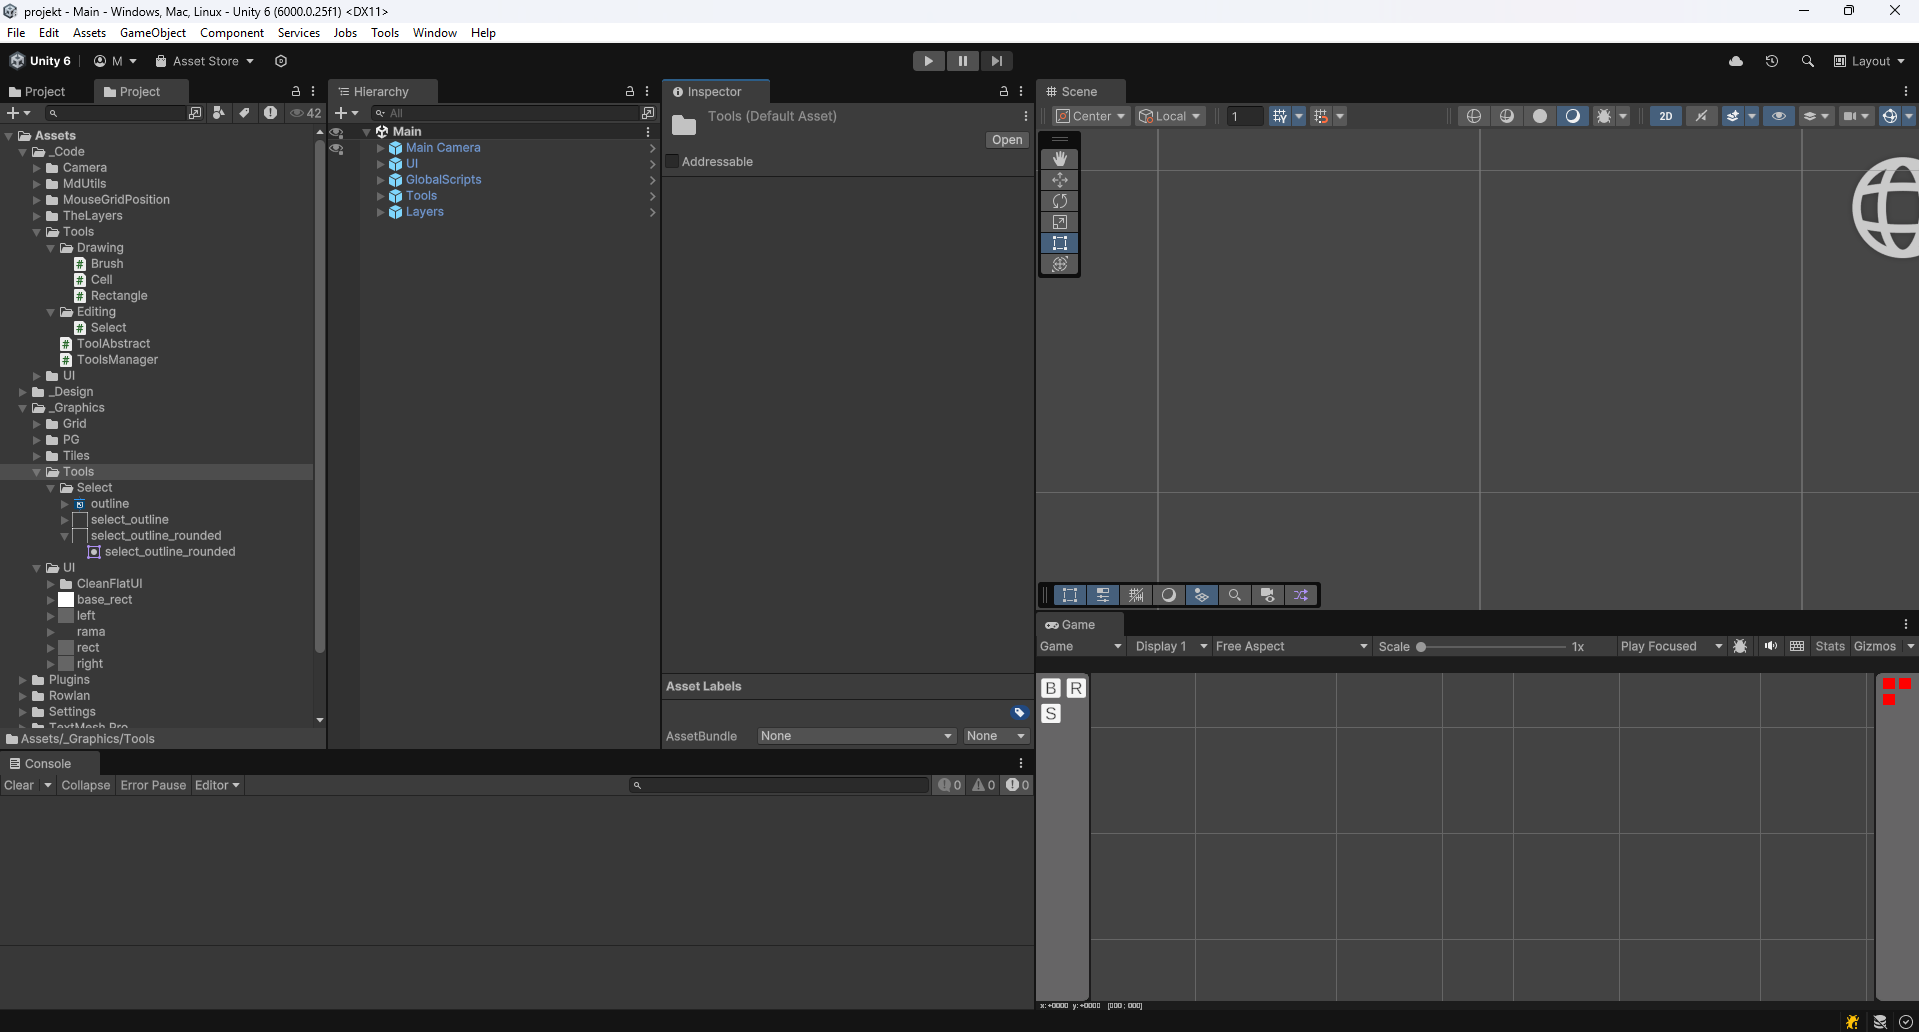
\includegraphics[width=0.9\textwidth]{chapters/chapter3/rys/unity_editor}
    \caption[Widok okna edytora Unity]{Wygląd edytora Unity, źródło: \cite{unity_site}}
    \label{fig:unity_editor}
\end{figure}

\subsection{Architektura programu}
\label{subsec:architektura_programu}

Aby zapewnić modularność oraz separację elementów aplikacji,
wykorzystano odpowiednio zaadaptowana architekturę MVVM (ang. Model-View-ViewModel).
Polega ona na podziale na trzy główne części: model, widok oraz widok-model.
Funkcje każdego z nich opisano w tab.~\ref{tab:mvvm}.

\begin{table}[h]
    \centering
    \caption[Opis funkcji poszczególnych elementów architektury MVVM.]
    {Opis funkcji poszczególnych elementów architektury MVVM, źródło:~\cite{mvvm}.}
    \label{tab:mvvm}
    \begin{tabular}{|c|p{0.6\textwidth}|}
        \hline
        Element & Opis \\
        \hline
        \hline
        Widok & Odpowiada za prezentację danych oraz interakcję z użytkownikiem. \\
        \hline
        Widok-model & Odpowiada za przekazywanie danych pomiędzy modelem a widokiem. \\
        \hline
        Model & Odpowiada za przechowywanie danych oraz logikę danego komponentu programu. \\
        \hline
    \end{tabular}
\end{table}

%Tak jak pierwotnie w architekturze MVVM,
%widok odpowiada za prezentację danych oraz interakcję z użytkownikiem.
%Przy czym po adaptacji widok-model odpowiada za nie tylko przekazywanie danych nie tylko między modelem a widokiem,
%ale również pomiędzy innymi częściami aplikacji jako menedżer danego systemu aplikacji.
%Sam model natomiast składa się z wielu komponentów, które przechowują dane oraz logikę danego komponentu aplikacji.
Przy większych projektach model ten jest stosowany do większości komponentów składających się na aplikację.
Widok-model w tej sytuacji odpowiada za przekazywanie danych nie tylko między modelem a widokiem,
ale również pomiędzy innymi częściami wewnątrz aplikacji jako menedżer danego systemu.
W przypadku opracowywanego programu można wyróżnić cztery główne systemy dotyczące różnych aspektów aplikacji:

\begin{citemize}
    \item System zarządzania progresem gry, odpowiadający za kontrolę przebiegu gry,
    a także punktację oraz weryfikację poziomów,
    \item Narzędzia do rysowania i edycji, wybieranie ich oraz kontrola ich działania,
    \item System zarządzania rysowanym schematem,
    odpowiadający za renderowanie warstw i przechowywanie informacji o nich
    oraz kontrolujący ich widok czy połączenia, na jakie się składają,
    \item System zapisu, odpowiadający za zapis i odczyt stanu gry.
\end{citemize}

%zarządzanie progresem gry, narzędzia do rysowania i edycji, system zarządzania rysowanym schematem, oraz system zapisu.
Odstępstwem od architektury MVVM jest natomiast potrzeba bezpośredniej interakcji pomiędzy użytkownikiem
a narzędziami ze względu na ich różnorodność, co przekłada się także na mniej skomplikowany kod.\\
Zarys architektury programu przedstawiono na rys.~\ref{fig:architektura}.

\begin{figure}[h!]
    \centering
    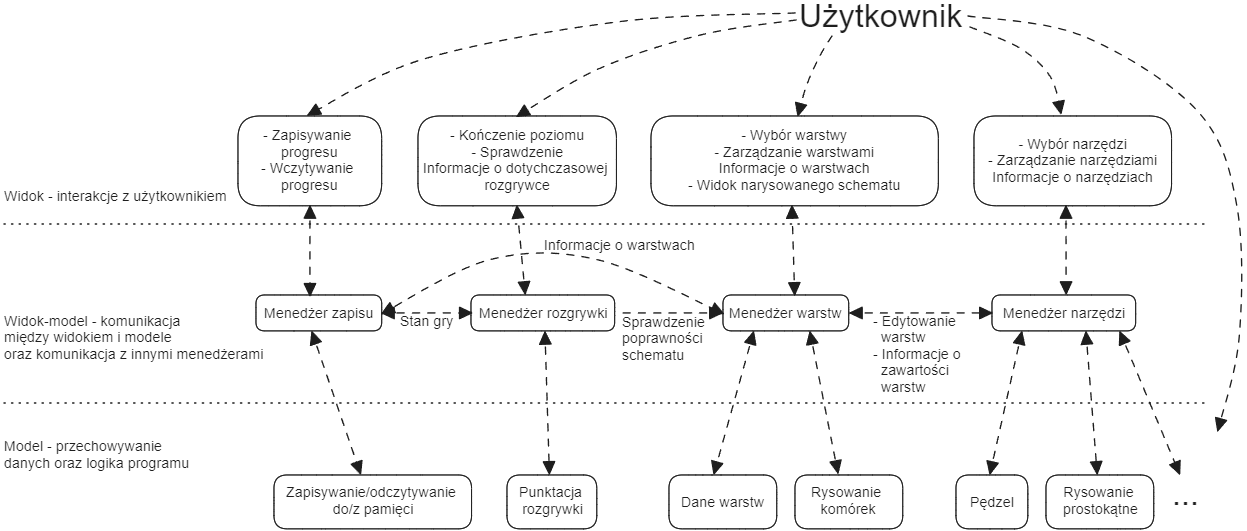
\includegraphics[width=\textwidth]{chapters/chapter3/rys/arch}
    \caption[Architektura programu.]{Architektura programu, źródło: opracowanie własne.}
    \label{fig:architektura}
\end{figure}

%\newpage % TODO: check this if something changes
\subsection{Wykorzystanie funkcji Unity oraz paczek zasobów}
\label{subsec:zasoby}

Do rysowania komórek schematów wykorzystano komponent \textit{SpriteRenderer},
pozwalający na renderowanie dwu-wymiarowych obrazów nazywanych \textit{sprite'ami}.
Dużą zaletą tego komponentu jest wbudowana optymalizacja ze strony Unity.
Obiektów tego typu może być wiele na scenie oraz są one renderowane tylko,
gdy są widoczne na ekranie~\cite{unity_csharp, unity_docs}. \\
\indent Prócz podstawowego skryptu, na jakim bazuje Unity, czyli \textit{MonoBehaviour},
wykorzystano także \textit{ScriptableObject}.
Jest to klasa, która pozwala na tworzenie obiektów, które mogą przechowywać dane zdefiniowane poza pracą programu,
a nawet wykonywać prostą logikę~\cite{unity_csharp, unity_docs}.
%Pozwala to na szczególną modularność dzięki możliwości wcześniejszego zdefiniowania danych zawartych w obiekcie
%i co mają one robić, a następnie tworzenie obiektów na ich podstawie.
Działanie SO jest zbliżone do klas i obiektów w OOP,
przy czym SO jest wykorzystywany przede wszystkim w edytorze Unity.
Dzięki temu można wcześniej zdefiniować jaki rodzaj danych powinien przechowywać dany typ obiektu,
a następnie tworzyć na ich podstawie konkretne instancje, których dane można zmieniać w edytorze.
Zostało to w szczególności wykorzystane w systemach zarządzania, rysowanym schematem
i narzędziami do rysowania i edycji.\\
%W przypadku schematu SO przechowuje informacje o tym jak powinny wyglądać i zachowywać się warstwy,
%natomiast do narzędzi SO zostały wykorzystane jako konfiguracje 
\indent W celu optymalizacji wskazane jest korzystanie z asynchroniczności w programie.
W szczególności jest to istotne podczas rysowania lub modyfikowania większych obszarów,
ponieważ wymaga to działania na wielu komórkach.
Skorzystano tutaj z paczki zasobów \textit{UniTask} do obsługi asynchroniczności,
dostępnej na platformie GitHub~\cite{unitask}.
Paczka ta adaptuje wbudowany w C\# system asynchroniczności,
dzięki czemu jest on znacznie optymalniejszy pod kątem wykorzystania w silniku Unity.


\subsection{Interfejs użytkownika}
\label{subsec:interfejs_uzytkownika}

Interfejs użytkownika (ang. \textit{User Interface}) jest jednym z kluczowych elementów każdej aplikacji,
kluczowe jest, aby był on intuicyjny oraz przejrzysty tak,
aby użytkownik mógł skupić się na korzystaniu z programu.
W przypadku opracowywanej aplikacji należy rozdzielić ją na dwie warstwy,
edytor schematów oraz część dotyczącą gry.
Jako że przez większość pracy w programie użytkownik ma do czynienia z edytorem schematów,
jest on podstawowym widokiem.
Z kolei elementy interfejsu dotyczące gry powinny być w formie nakładki na edytor schematów,
z wyjątkiem okna startowego, który będzie odrębną sceną, przez co nie ma potrzeby tworzenia nakładki.
Zarys widoku okna edytora schematów przedstawiono na rys.~\ref{fig:editor}.

\begin{figure}[h]
    \centering
    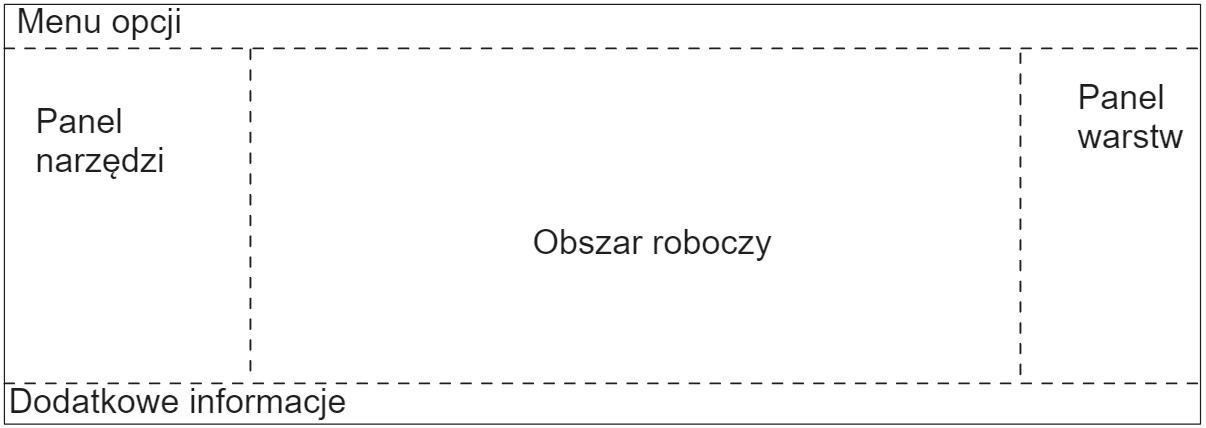
\includegraphics[width=0.89\textwidth]{chapters/chapter3/rys/ui_projekt}
    \caption[Szkic okna edytora schematów]{Szkic okna edytora schematów, źródło: opracowanie własne.}
    \label{fig:editor}
\end{figure}

\indent Okno dla edytora adaptuje elementy
z programów wspomnianych w rozdziale~\ref{ch:przeglad_istniejacych_rozwiazan}.
Tak jak w przypadku większości rozwiązań u góry okna znajduje się pasek opcji programu,
implementujący również opcje związane z grą.
Poniżej znajduje się obszar roboczy, gdzie użytkownik może rysować schematy.
Na dole okna znajduje się pasek informacyjny, który zawiera dane o aktualnie wybranym narzędziu,
a także o możliwych dodatkowych akcjach do wykonania.
Z prawej strony okna znajduje się panel warstw, zawierający dostępne warstwy schematu,
a także dodatkowe informacje o nich wraz z możliwością wyłączenia ich widoczności.
Po lewej usytuowany jest panel narzędzi, zawierający dostępne funkcje rysowania i edycji schematów
i dostępne dla nich opcje.
